\documentclass[12pt]{extarticle}

% ------------- [ METADATA ] -------------
\begin{filecontents*}[overwrite]{\jobname.xmpdata}
  \Title{
    Tecnologie informatiche per il Web – IntelliJ Guide
  },
  \Author{Vittorio Robecchi},
  \Producer{LuaLaTeX},
  \Creator{LaTeX},
\end{filecontents*}
\usepackage{setspace}
\PassOptionsToPackage{
  hyperfootnotes=true,
  colorlinks=true,
  linkcolor=red,
  citecolor=blue,
  filecolor=blue,
  urlcolor=blue,
}{hyperref}
\usepackage[a-3u]{pdfx} % PDF/A - 3u

\usepackage[paper=a4paper,margin=2cm]{geometry}
\usepackage{listings}
\usepackage{minted} % python-pigments needed
\usepackage{graphicx}
\usepackage{float}
\usepackage[T1]{fontenc}
\usepackage{cleveref}
\usepackage[indent]{parskip}
\usepackage{xcolor}
\usepackage[framemethod=TikZ]{mdframed}

\newenvironment{hint}[2][]{%
  \mdfsetup{skipabove=10pt,frametitle={%
      \tikz[baseline=(current bounding box.east),outer sep=0pt]
      \node[anchor=east,rectangle,fill=blue!20]
  {#1};}}%
  \mdfsetup{innertopmargin=2pt,linecolor=blue!20,%
    linewidth=2pt,topline=true,%
    frametitleaboveskip=\dimexpr-\ht\strutbox\relax
  }
  \begin{mdframed}[]\relax%
  \label{#2}}{
\end{mdframed}}

\newenvironment{tip}[2][]{%
  \mdfsetup{skipabove=10pt,frametitle={%
      \tikz[baseline=(current bounding box.east),outer sep=0pt]
      \node[anchor=east,rectangle,fill=orange!20]
  {#1};}}%
  \mdfsetup{innertopmargin=2pt,linecolor=orange!20,%
    linewidth=2pt,topline=true,%
    frametitleaboveskip=\dimexpr-\ht\strutbox\relax
  }
  \begin{mdframed}[]\relax%
  \label{#2}}{
\end{mdframed}}

\newenvironment{warning}[2][]{%
  \mdfsetup{skipabove=10pt,frametitle={%
      \tikz[baseline=(current bounding box.east),outer sep=0pt]
      \node[anchor=east,rectangle,fill=red!20]
  {#1};}}%
  \mdfsetup{innertopmargin=2pt,linecolor=red!20,%
    linewidth=2pt,topline=true,%
    frametitleaboveskip=\dimexpr-\ht\strutbox\relax
  }
  \begin{mdframed}[]\relax%
  \label{#2}}{
\end{mdframed}}

\newcommand\red[1]{\textcolor{red}{#1}}

\title{
  Tecnologie informatiche per il Web \\
  % \rule{0.5\textwidth}{1pt} \\
  IntelliJ Guide
}
\date{}

\begin{document}
\maketitle
\tableofcontents

% ad ogni sezione, vai a capo
\let\latexsection\section
\renewcommand{\section}{
  \newpage
  \latexsection
}

% sections
\section{Preliminaries}

The tech stack is as follows:
\begin{itemize}
  \item IntelliJ Idea Ultimate as Java IDE and Maven as build system
    \begin{itemize}
      \item Datagrip as SQL IDE
    \end{itemize}
  \item MariaDB, a retrocompatible fork of MySQL
  \item Tomcat as application server
\end{itemize}

\begin{hint}[OS compatibility]{}
  Although the guide has been verified on Arch Linux, since all of JetBrains' IDEs are cross-platform, apart from the installation process, commands and paths the configuration will be the same on \textit{every} operating system.
\end{hint}

Programs and dependencies needed:
\begin{minted}{shell}
  # from ufficial repositories
  sudo pacman -S jdk21-openjdk mariadb tomcat10 maven

  # from AUR
  yay -S intellij-idea-ultimate-edition mariadb-jdbc
\end{minted}

to install \texttt{yay} check the \href{https://github.com/Jguer/yay?tab=readme-ov-file#installation}{official repository}.

All of Datagrip functionalities are integrated in every JetBrains' IDE, so its not stricly needed -- however, if you want install Datagrip as a standalone application:
\begin{minted}{shell}
  # from AUR
  yay -S datagrip datagrip-jre
\end{minted}

\section{IntelliJ Idea configuration}

\begin{enumerate}
  \item Create a new project with \texttt{Jakarta EE} as generator:
    \begin{itemize}
      \item Template: web application
      \item JDK: OpenJDK 21 (path: \texttt{/usr/lib/jvm/java-21-openjdk})
      \item Build system: Maven\footnote{In accordance with the Software Engineering course.}
        \begin{figure}[H]
          \centering
          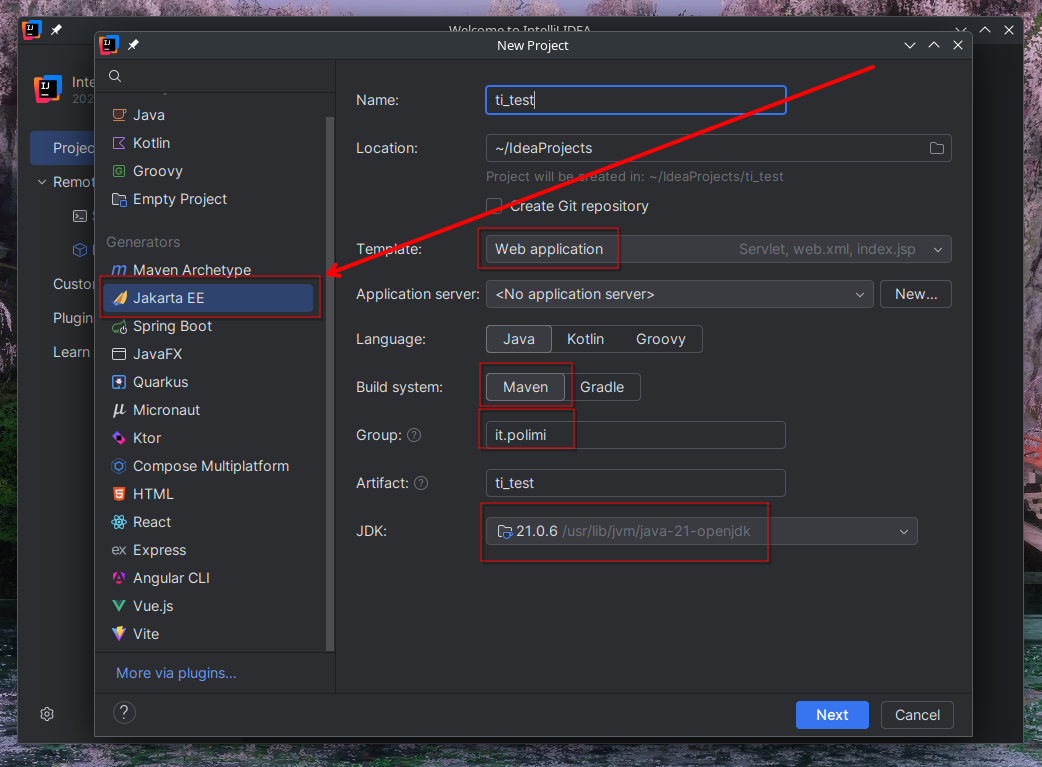
\includegraphics[width=0.6\textwidth]{img/intellij/intellij_2.png}
          \caption{IntelliJ project configuration.}
        \end{figure}

        % \newpage
      \item Application server: Tomcat (path: \texttt{/usr/share/tomcat10})
        \begin{figure}[H]
          \centering
          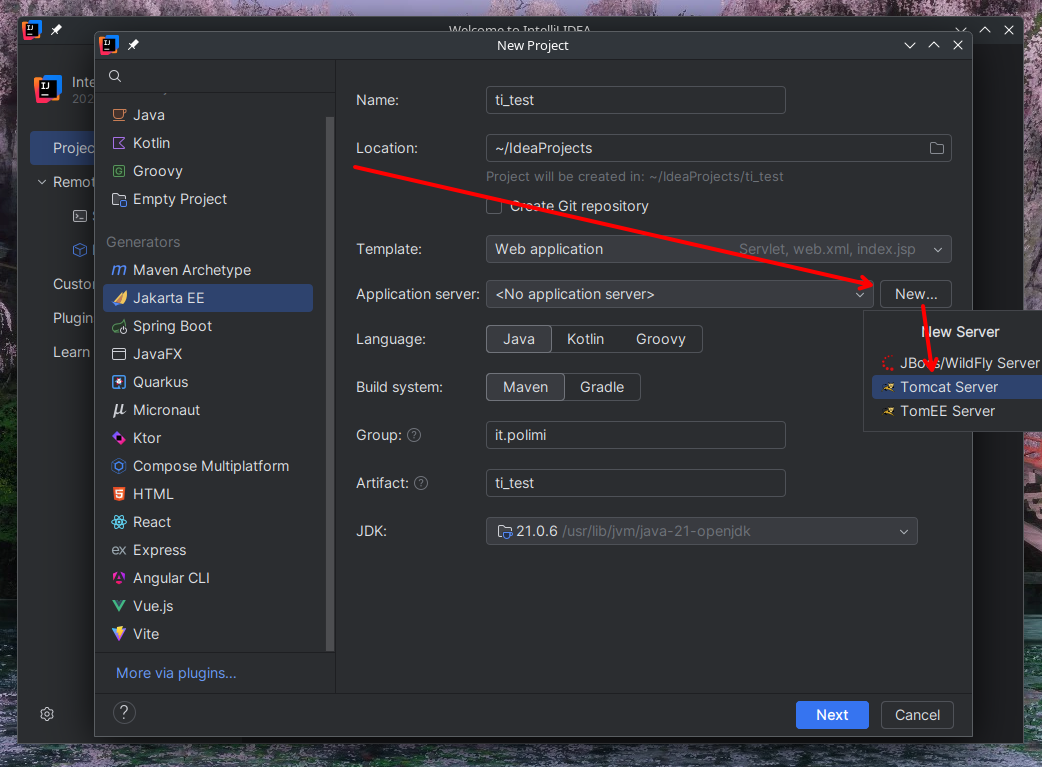
\includegraphics[width=0.6\textwidth]{img/intellij/intellij_3.png}
          \caption{Tomcat configuration (1/2).}
        \end{figure}

        \begin{figure}[H]
          \centering
          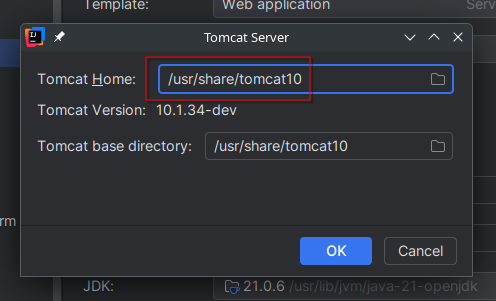
\includegraphics[width=0.45\textwidth]{img/intellij/intellij_4.png}
          \caption{Tomcat configuration (2/2).}
        \end{figure}
    \end{itemize}
  \item Check Eclipse server and client, Welde as implementations
    \begin{figure}[H]
      \centering
      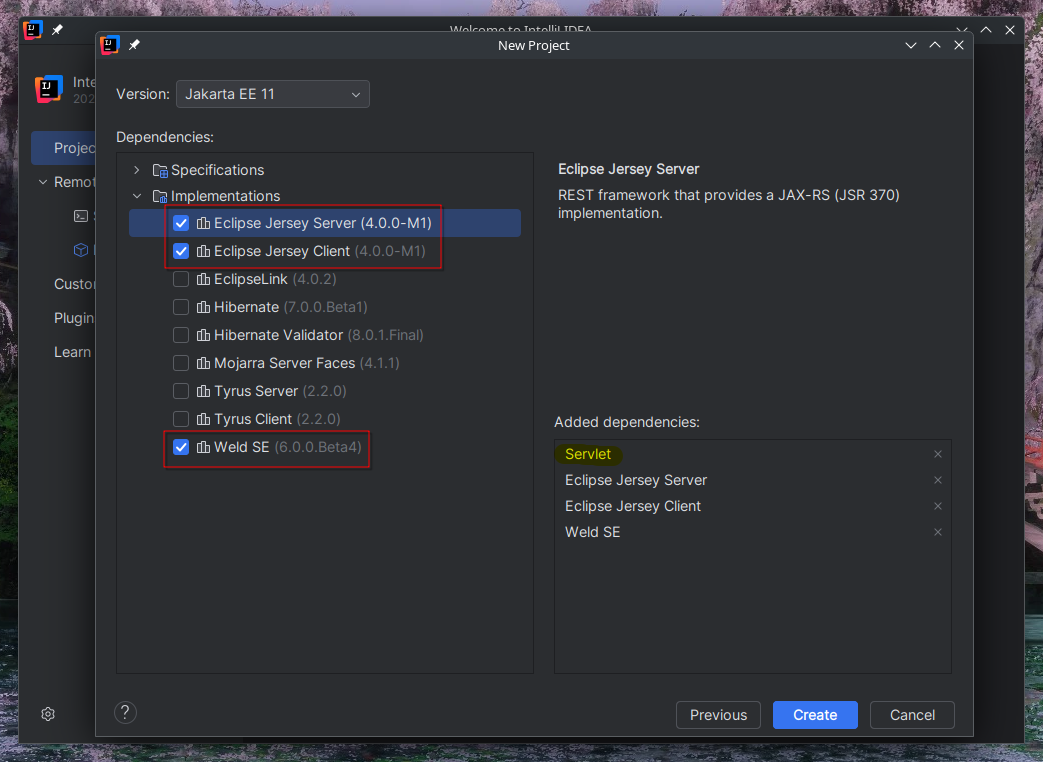
\includegraphics[width=0.6\textwidth]{img/intellij/intellij_5.png}
    \end{figure}
    note that Servlet is already added as dependency.
\end{enumerate}

\begin{tip}[Permissions error]{}
  After a test, IntelliJ could report an error stating it cannot copy \texttt{/usr/share/tomcat10/conf} -- this maybe caused by permissions:
  \begin{figure}[H]
    \centering
    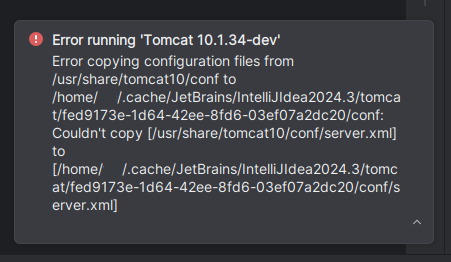
\includegraphics[width=0.5\textwidth]{img/intellij/intellij_6.png}
    \caption{IntelliJ error.}
  \end{figure}
  \newpage
  to fix it run:
    \begin{minted}{shell}
      sudo chmod -R 777 /usr/share/tomcat10/conf
    \end{minted}
\end{tip}

\subsection{Database configuration}\label{sec: db_intellij}

\begin{enumerate}
  \item Configure MariaDB
    \begin{minted}{shell}
    mariadb-install-db --user=mysql --basedir=/usr --datadir=/var/lib/mysql
    mariadb-secure-installation
    \end{minted}
    and then start it:
    \begin{minted}{shell}
    sudo systemctl start mariadb
    \end{minted}
    If you want to start the database server at every boot type:
    \begin{minted}{shell}
    sudo systemctl enable mariadb
    \end{minted}

  \item Create the user and grant \emph{all} permissions on \emph{all} databases:
    \begin{minted}{shell}
    sudo mariadb
    MariaDB [(none)]> CREATE USER 'name'@'localhost' IDENTIFIED BY 'password';
    MariaDB [(none)]> GRANT PRIVILEGES ON *.* TO 'name'@'localhost';
    MariaDB [(none)]> quit;
    \end{minted}
    this is needed since in order to create a database \emph{you need permission} to do so. If you want to check:
    \begin{minted}{shell}
    MariaDB [(none)]> SHOW ALL PRIVILEGES FOR 'name'@'localhost';
    \end{minted}

  \item Open the database configuration from IntelliJ (above right)
    \begin{figure}[H]
      \centering
      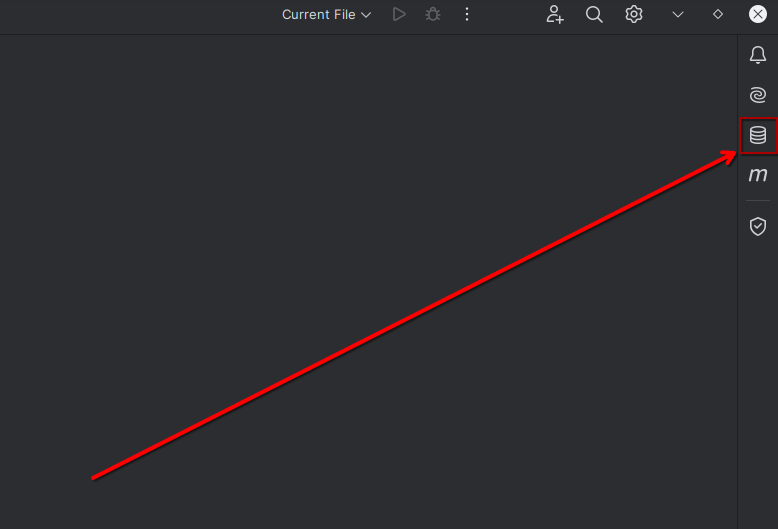
\includegraphics[width=0.6\textwidth]{img/intellij/intellij_8.png}
      \caption{Database configuration in IntelliJ.}
    \end{figure}

  \item To import a MySQL dump execute the following command:
    \begin{minted}{shell}
    mariadb --user name --password < dump.sql
    \end{minted}
    where \texttt{name} and \texttt{password} reference step 2.

    \newpage

  \item From the above left menu add the data source:
    \begin{itemize}
      \item Select MariaDB
        \begin{figure}[H]
          \centering
          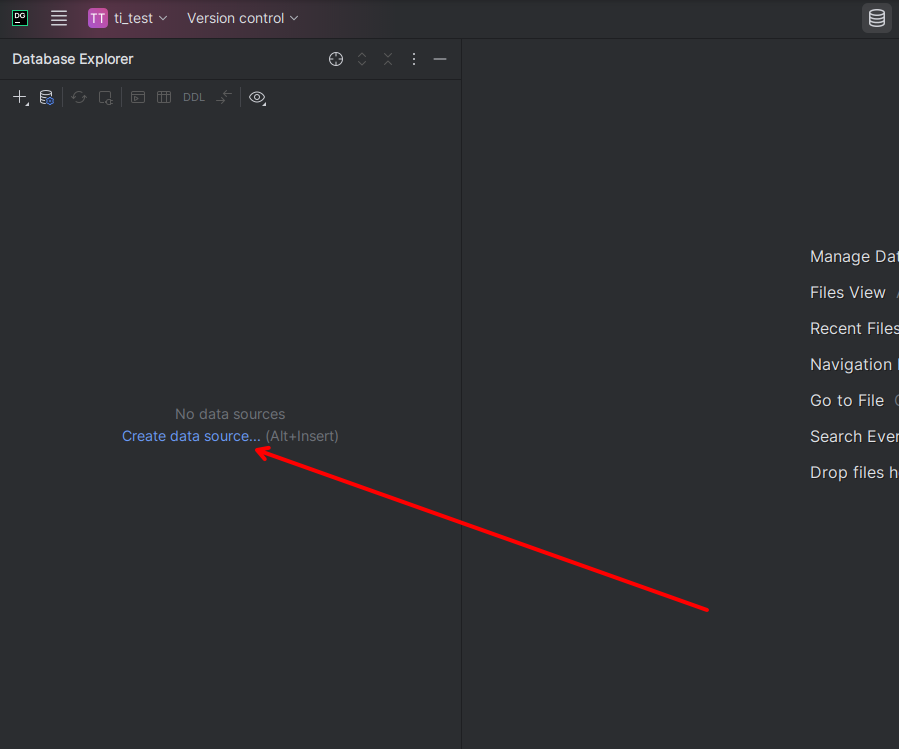
\includegraphics[width=0.49\textwidth]{img/datagrip/datagrip_2.png}
          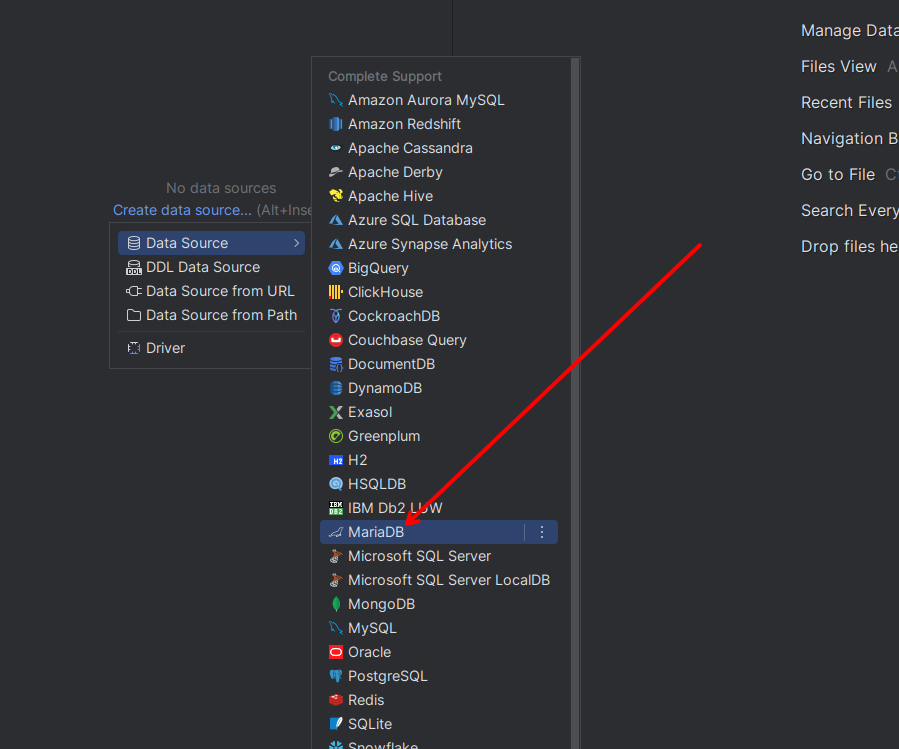
\includegraphics[width=0.49\textwidth]{img/datagrip/datagrip_3.png}
          \caption{Selecting MariaDB as source.}
        \end{figure}
      \item \texttt{user}, \texttt{password} from step 2
      \item Name of the database from step 5 -- to see available databases:
    \begin{minted}{shell}
    sudo mariadb
    MariaDB [(none)]> SHOW DATABASES;
    MariaDB [(none)]> quit;
    \end{minted}
    \end{itemize}
    \begin{figure}[H]
      \centering
      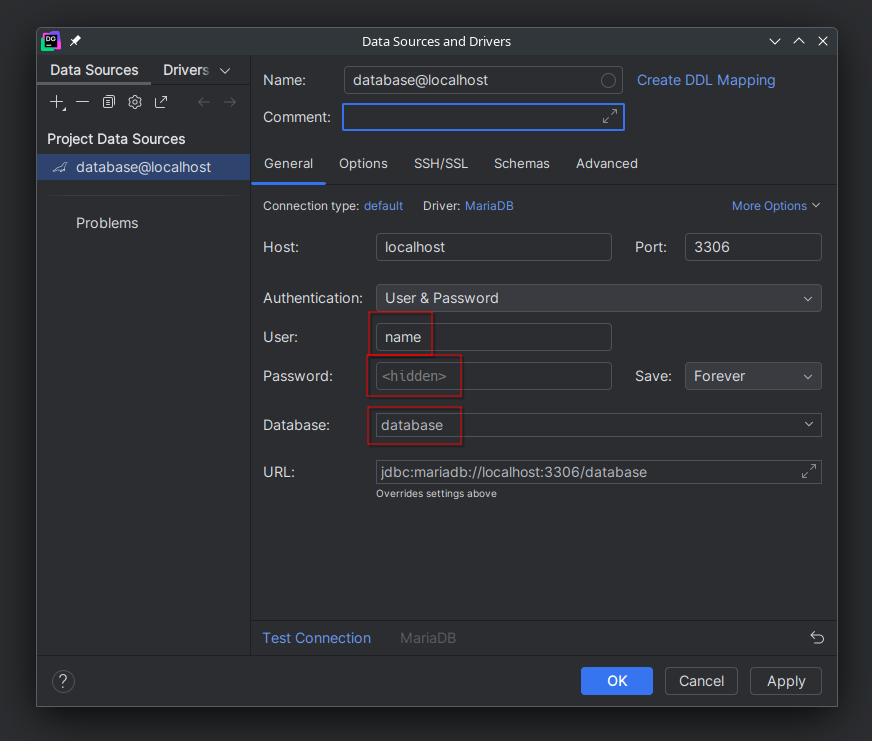
\includegraphics[width=0.6\textwidth]{img/datagrip/datagrip_4.png}
      \caption{Adding the database.}
    \end{figure}
\end{enumerate}

Repeat step 4 and 5 for each dump.

\newpage

\subsection{Configure MariaDB connection}

Add the following to \texttt{pom.xml}:
\begin{minted}{xml}
  <dependency>
   <groupId>org.mariadb.jdbc</groupId>
   <artifactId>mariadb-java-client</artifactId>
   <version>3.4.1</version>
  </dependency>
\end{minted}
and synchronize Maven, which then adds all the necessary drivers. Last but not least, verify the connection by creating the \texttt{ConnectionTester} class:
\begin{minted}{java}
  import java.sql.*;

  public class ConnectionTester {
    public static void main(String[] args) throws SQLException,
    ClassNotFoundException {
      final String DATABASE = "database";
      final String USER = "name";
      final String PASSWORD = "password";
      Connection connection = null;

      // Load the JDBC driver
      try {
          Class.forName("org.mariadb.jdbc.Driver");
          System.out.println("Driver loaded");
      } catch (ClassNotFoundException e) {
          System.err.println("Driver not found");
          e.printStackTrace();
      }
      try {
          connection = DriverManager.getConnection
                  ("jdbc:mariadb://localhost:3306/" + DATABASE, USER, PASSWORD);
          System.out.println("Database connection successful");
          connection.close();
      } catch (Exception e) {
          System.err.println("Connection failed");
          e.printStackTrace();
      }
    }
  }
\end{minted}
by editing \texttt{DATABASE}, \texttt{USER} and \texttt{PASSWORD} accordingly.

\subsection{Configure Maven dependencies}

In order to make the current Eclipse projects to work, the \texttt{pom.xml} file needs some other dependencies:
\begin{minted}{xml}
<dependencies>
    <!-- Jakarta EE servlet (jsp, jstl) -->
    <dependency>
        <groupId>org.glassfish.web</groupId>
        <artifactId>jakarta.servlet.jsp.jstl</artifactId>
        <version>2.0.0</version>
    </dependency>
    <dependency>
        <groupId>jakarta.servlet.jsp.jstl</groupId>
        <artifactId>jakarta.servlet.jsp.jstl-api</artifactId>
        <version>2.0.0</version>
    </dependency>
    <!-- Thymeleaf -->
    <dependency>
        <groupId>org.thymeleaf</groupId>
        <artifactId>thymeleaf</artifactId>
        <version>3.1.3.RELEASE</version>
    </dependency>
</dependencies>
\end{minted}

\textbf{Be sure} to use the correct versions. Search them on the Maven repository with the following URL scheme: \texttt{https://mvnrepository.com/artifact/\red{groupId}/\red{artifactId}}.

Also, you might need to set the JDK version:
\begin{minted}{xml}
    <properties>
        <!-- Properties set for Java 21 -->
        <maven.compiler.source>21</maven.compiler.source>
        <maven.compiler.target>21</maven.compiler.target>
        <project.build.sourceEncoding>UTF-8</project.build.sourceEncoding>
    </properties>
\end{minted}

\begin{warning}[Follow the standard structure]{}
  Finally, the directory tree will have to look like:
    \begin{verbatim}
    src/
    |-- main/
    |   |-- java/
    |   |   `-- it.polimi.tiw
    |   |-- resources
    |   `-- webapp
    `-- test/
        |-- java/
        |   `-- it.polimi.tiw
        |-- resources
        `-- webapp
    LICENSE.txt
    README.md
    pom.xml
    \end{verbatim}

  In accordance with the \href{https://maven.apache.org/guides/introduction/introduction-to-the-standard-directory-layout.html}{Maven standard directory layout}.

  This is \textbf{not optional}: for instance, in some projects there's a \texttt{resources} folder which is NOT located in the correct path; once the project will be deployed, Java will look for the \texttt{src/main/resources} folder and will not find it. IntelliJ won't throw an error.
\end{warning}

\section{Datagrip configuration}

\begin{enumerate}
  \item Follow step 1, 2 from \autoref{sec: db_intellij}
  \item Create a new project in Datagrip
    \begin{figure}[H]
      \centering
      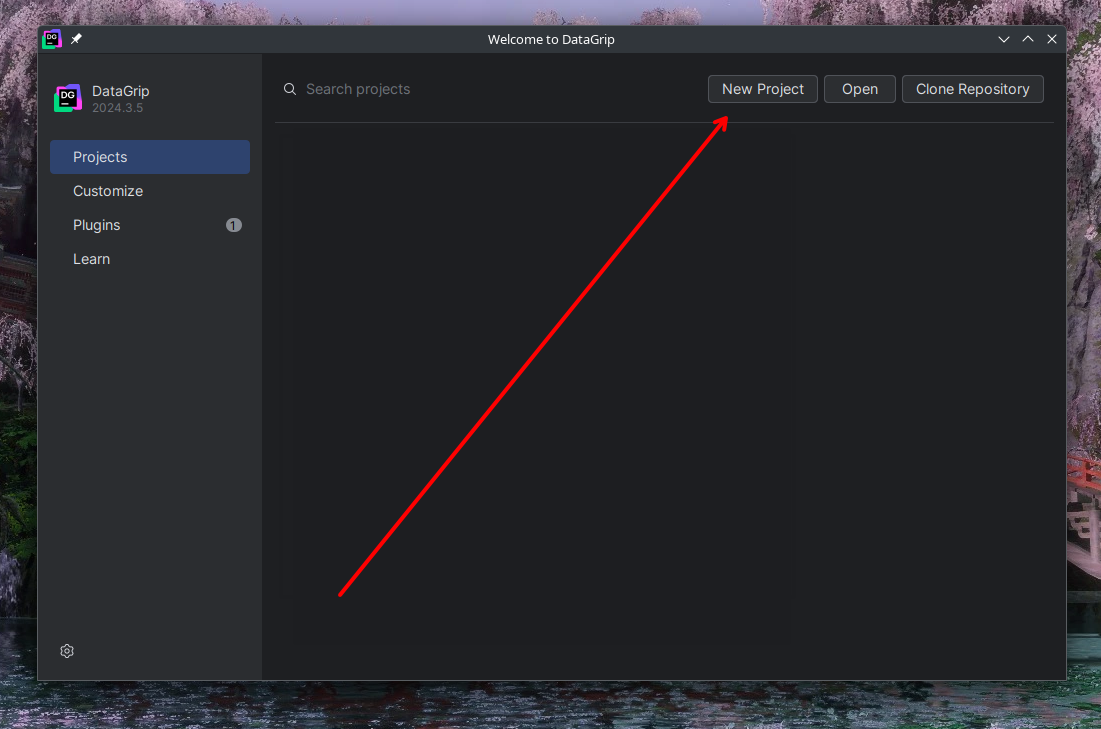
\includegraphics[width=0.6\textwidth]{img/datagrip/datagrip_1.png}
      \caption{Creating a new project in Datagrip.}
    \end{figure}

  \item Follow the remaining steps from \autoref{sec: db_intellij}
\end{enumerate}


\end{document}